% !TEX root = ../../../main/aws_chabauty.tex
\newpage
\section{Bjorn Poonen: Introduction to Chabauty's method and Kim's nonabelian generalization}
\subsection{Lecture 1}
\subsubsection{Rational points on Curves}

The starting point is Falting's Theorem, which was originally Mordell's conjecture.

\begin{thm}[Falting's, 1983]
Suppose $[K \colon \Q] < \infty$.
$X$ a `nice'\footnote{smooth, projective, geometrically integral} curve of genus $g$ over $K$. If $g>1$, then $X(K)$ is finite. 
\end{thm}


There are several proofs now. The first was Falting's proof in 1983 based on Arakelov methods. The next was by Vojta 1991 and its variant (phrased in more elementary terms via Diophantine approximation) by Bomberi. But now there is a proof by Lawrence-Venkatesh in 2018 via $p$-adic period maps. 


For integral points, the parallel to Falting's Theorem is Siegel's Theorem. Let $[K \colon \Q] < \infty$. Let $\O= \O_{K,S}= \{ x \in K \colon \nu(x) \geq 0 \text{for all } \nu \in S \}$, where $S$ is a finite set of places, including all the archimedean places. Let $U:= X \setminus Z$, where $X$ is a nice curve of genus $g$ and $Z$ is a nonempty 0-dimensional subscheme. Now $\chi(U):= (2-2g) - r$, where $r= \#Z(\overline{K})$ and $\chi$ is the Euler characteristic. Suppose $\cU$ is a finite type $\O$-scheme with $\cU_K= U$. If $\chi(U)< 0$. The condition that $\chi(U)<0$ is sometimes phrased as that $U$ is hyperbolic [over $\C$, $\widetilde{U} \simeq b$]. 


\begin{thm}[Siegel's Theorem]
If $\chi(U)< 0$, then $\cU(\O)$ is finite. 
\end{thm}


There is a proof, obviously, by Siegel. But there are proofs by Baker-Coates (1970) when either $g \leq 1$ or when $U$ is $y^2= f(x)$ in $\A^2$ and Lawrence-Venkatesh (2018) when $I= \P^1 \setminus \{0,1,\infty\}$. 


\begin{ex}
If $U= \P \setminus \{0,1,\infty\}$, then $\cU= \spec \O[x, \frac{1}{x},\frac{1}{1-x}]$ and $\cU(\O)$ is the set of solutions to $x+y=1$ with $x,y \in \O^\times$. 
\end{ex}


\begin{rem}
Falting's Theorem is strictly harder than Siegel's Theorem in that Falting's Theorem implies Siegel's Theorem. The key idea is that if $\chi(U)<0$, then there is some finite \etale cover of $U$ is open in a nice curve of genus greater than 1.  
\end{rem}


In Siegel-Falting, $\chi(U)<0$ means that 


\begin{itemize}
\item $g=0$, then $r \geq 3$
\item $g=1$, then $r \geq 1$
\item $g \geq 2$, $r$ arbitrary 
\end{itemize}


The problem with nearly all of these methods is that they are not effective. The goal is then to try to make them effective. This was exactly the hope of Chabauty. 



% Chabauty's Method
\subsubsection{Chabauty's Method}

	\[
	\begin{tikzcd}
	K \arrow[dash,swap]{d}{[K\,:\,\Q]=\,\dim_\Q K} & \p \\
	\Q & p 
	\end{tikzcd}
	\]

Let $X$ be a nice curve of genus $g$ over $K$. Then $X$ is a $g$-dimensional abelian variety. Let $J= \jac  X$ and let $r= \rank J(K)$. Choose $x \in X(K)$ to get $X \hookrightarrow J$. 

% Picture
	\begin{figure}[!ht]
	\centering 
	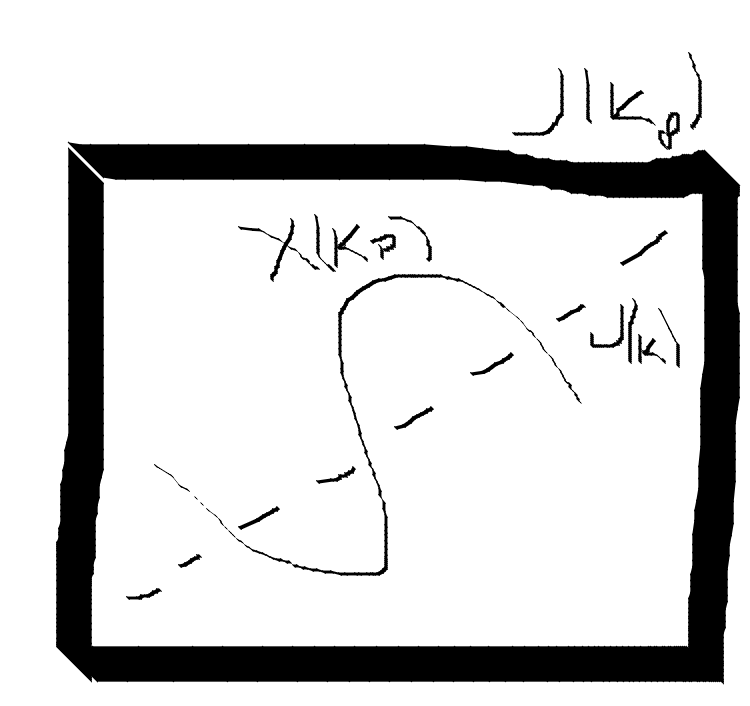
\includegraphics[width=0.3\textwidth]{../images/im1.png}
	\end{figure}
	
%	\[
%	\begin{tikzpicture}
%	\begin{axis}[]
%	\addplot[domain=0:2*pi, samples=50, black] ({\x},{\x});
%	\end{axis}
%	\end{tikzpicture}
%	\]

	\[
	\begin{tikzcd}
	X(K) \arrow{r} \arrow{d} &  X(K_\p) \arrow{d} \\
	J(K) \arrow{r} & J(K_\p) \arrow{r}{\log} & \lie J_{K_\p} \simeq K_\p^g
	\end{tikzcd}
	\]

The kernel of the log map is finite and is a local diffeomorphism so the image will be open and compact ($J$ is a compact group). Therefore, the image of log is an open compact subgroup of the Lie group $\lie J_{K_\p}$. Moreover, the image of $J(K) \to K_\p^g$ is generated by $r$ elements. Then the dimension of $K_\p$-span of the image is at most $r$. If $r< g$, there exists a nonzero linear $\lambda: \lie J_{K_\p} \to K_\p$ vanishing in $J(K)$, and $\lambda$ pulls back to a nonzero locally analytic function on $X(K_\p)$ vanishing on $X(K)$, so $X(K)$ is finite. But of course, this all requires what might be called Chabauty's condition: $r<g$. 


How do we limit the role of the Jacobian in this to generalize? Rewriting
	\[
	\begin{tikzcd}
	X(K) \arrow{d} \arrow{r} & X(K_\p) \arrow{d} \\
	J(K) \arrow{r} \arrow{d} & J(K_\p) \arrow{r}{\log} \arrow{d} & \lie J_{K_\p} \\
	\widehat{J(K)}[\frac{1}{p}] \arrow{r} & \widehat{J(K_\p)}[\frac{1}{p}] \arrow{ur}{\rotatebox{45}{$\sim$}} 
	\end{tikzcd}
	\]
Given $M$, an abelian group, define $\hat{M}:= \plim M/p^nM$, which is a $\Z_p$-module. Then $\hat{M}[\frac{1}{p}] \simeq \hat{M} \otimes_{\Z_p} \Q_p$, which is a $\Q_p$ vector space. 


$V$ is \etale homology. As a motivation, if $X$ is a curve over $\C$ and $J$ is its Jacobian. Then analytically, $J(\C) \simeq \C^g/ \Lambda$, where $\Lambda= H_1(J(\C),\Z)$. Using the right hand side, it is easy to see that 
	\[
	J[p] \simeq \frac{1}{p} \Lambda/\Lambda \ma{p} \Lambda/p\Lambda= H_1(J(\C), \Z/p\Z)= H_1(X(\C),\Z/p\Z) 
	\]
If we are not using $\C$, we are going to have to switch to \Etale (co)homology.


For $X$ over $K$, $J[p] \simeq H_1^\et(X_{\ov{K}}, \Z/p\Z):= \Z/p\Z$-dual of $H^1_\et(X_{\ov{K}}, \Z/p\Z)$. Likewise, $J[p^n] \simeq H_1^\et(X_{\ov{K}}, \Z/p^n\Z)$. Now $\Z_p$ is the Tate module, where $T:= \plim J[p^n] \simeq H_1^\et(X_{\ov{K}}, \Z_p)$. Tensoring with $\Q_p$, we obtain the $\Q_p$-Tate module $V:= T[\frac{1}{p}]= T \otimes_{\Z_p} \Q_p \simeq H_1^\et(X_{\ov{K}}, \Q_p)$, which is a $\Q_p$-vector space of dimension $2g$. 


Now write $\cV(\Q_p)$ for a group variety $\cV \simeq \G_a^{2g}$ over $\Q_p$. Note that $\cV$ is $\A^{2g}$ with an additive group law. The group $G_K:= \Gal(\ov{K}/K)$ acts continuously on all of these, e.g. $G_K \to \Aut \cV \simeq \GL_n(\Q_p)$, as a group variety. 

























